\chapter{光的直线传播}\label{ch:g6:light-propagation}

“光沿直线传播”这句话陪伴你们已有两年，
--- 照亮影子、瞄准镜子、将三张卡片与一支
蜡烛对齐。本学年，这条旧定律将获得正式名称、作图规则，
以及它最神奇的推论：一台没有透镜、没有玻璃、
也没有活动部件的相机 --- 只需一个小孔。

\section{正式表述的定律}

\begin{proposition}[光的直线传播]\label{prop:g6:light-propagation:law}
在洁净的空气中 --- 以及任何清澈、混合均匀的介质中，如
静水或玻璃 --- 光沿直线传播。这
这就是\emph{光的直线传播}\index{光的直线传播}的定律：
\emph{直线的}只是拉丁风味的词，意为
“直线形的”，而\emph{传播}一词指光
从一处到另一处的行进。
\end{proposition}

\begin{definition}[光线与光束]\label{def:g6:light-propagation:ray}
\emph{光线}\index{光线}是物理学家对一根光的图示：
一条带箭头的直线，箭头指示
其传播方向。真实的灯会同时发出无数根光线，
它们合起来的集合称为\emph{光束}\index{光束}。三种常见光束形状
足以涵盖实际：\emph{发散的}（光线自一点向外散开 ---
任何小灯都是如此），\emph{平行的}（光线并排，
既不相交也不分开 --- 经过远途的阳光），
以及\emph{会聚的}（光线向一点靠拢 ---
由你两年后将接触的仪器所汇集的光）。
\end{definition}

\begin{omfigure}
\begin{tikzpicture}[scale=0.8]
  \fill[omThm] (0.5,1.3) circle (0.14);
  \foreach \a in {-28,-14,0,14,28} {
    \draw[-Stealth, omThm, thick] (0.6,1.3) -- ++(\a:2.6);
  }
  \node[below, font=\small] at (1.8,-0.1) {发散};
  \foreach \y in {0.5,1.0,1.5,2.0} {
    \draw[-Stealth, omThm, thick] (4.6,\y) -- (7.4,\y);
  }
  \node[below, font=\small] at (6.0,-0.1) {平行};
  \foreach \a in {152,166,180,194,208} {
    \draw[-Stealth, omThm, thick] (11.4,1.3) ++(\a:2.6)
      -- ++({\a-180}:2.35);
  }
  \fill[omExo] (11.4,1.3) circle (0.1);
  \node[below, font=\small] at (9.8,-0.1) {会聚};
\end{tikzpicture}

{\small 三束光：自小灯发散而出，平行地来自
遥远的太阳，以及向一点会聚。}
\end{omfigure}

\begin{omfigure}
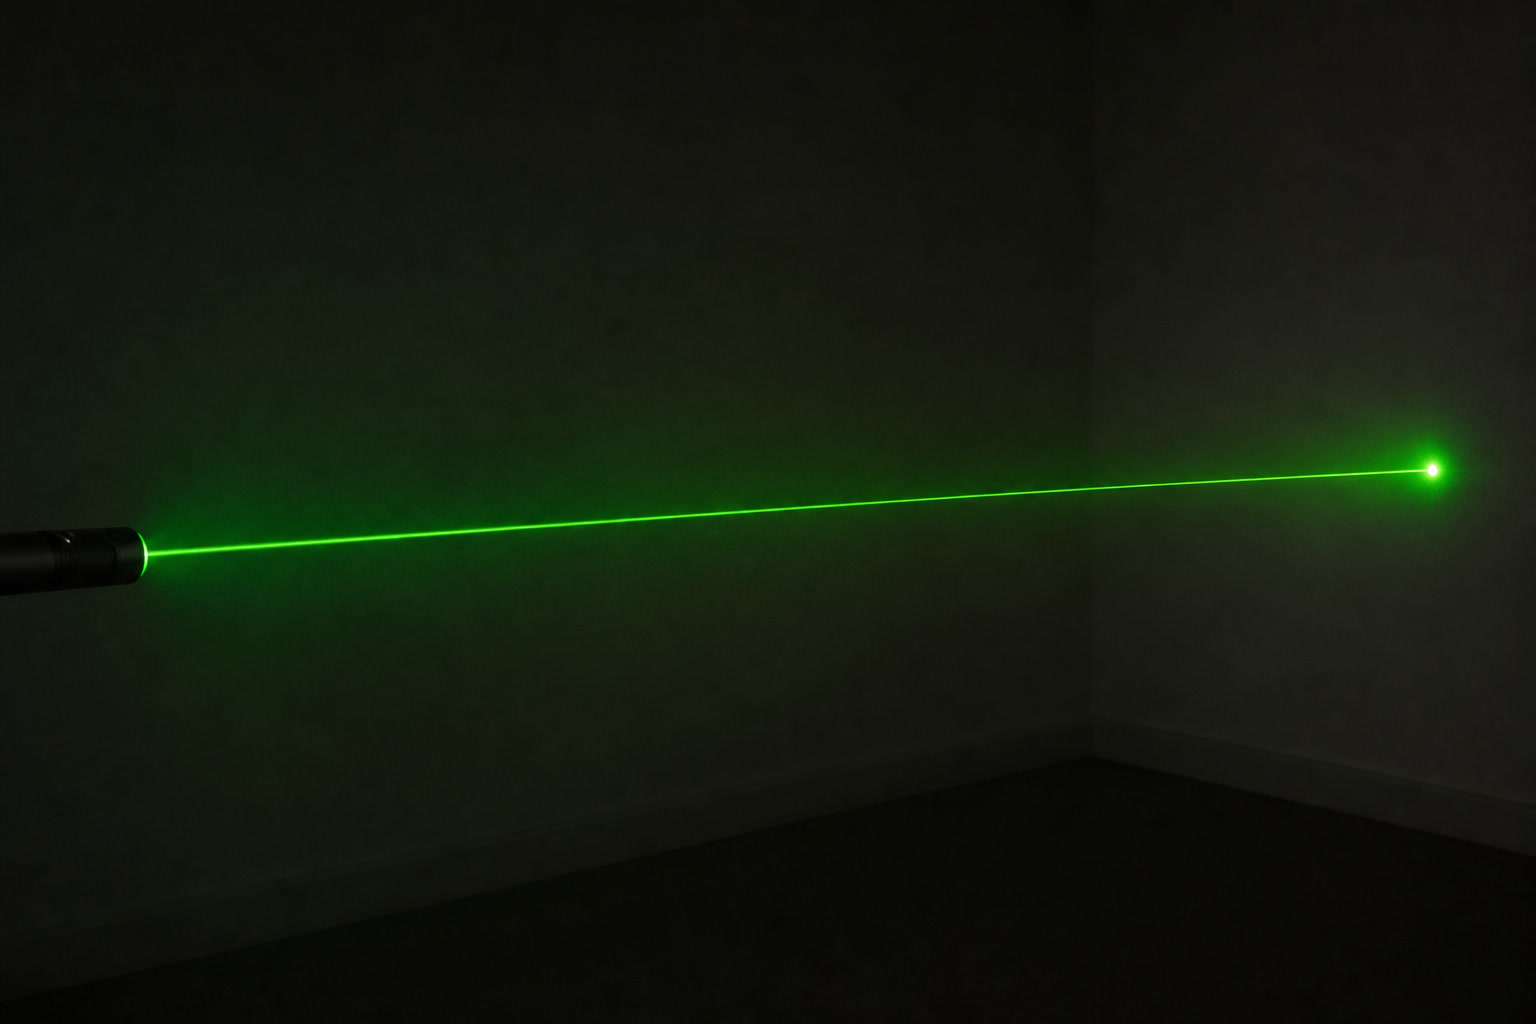
\includegraphics[width=0.55\linewidth]{images/book1/ai/g6-light-laser-fog.jpg}

{\small 雾气使激光束可见：从光源到墙壁是一条笔直的线。}
\end{omfigure}

\begin{example}[定律处处可见]\label{ex:g6:light-propagation:sightings}
木匠沿直木板的边缘瞄准以判断其平直 --- 眼睛、
边缘与远端须成一线，光的直线性正是
这一判断的依据。测量员用眼睛把标杆排成一线；射箭者与
摄影师“对准拍摄”；而两年前的三张卡片实验，
如今有了正式名称：一项对直线传播的检验。
这些做法都是用一条光的直线，
去对准一条实物的直线。
\end{example}

\section{作图求影子}

\begin{method}[用直尺作出影子]\label{met:g6:light-propagation:shadow}
对于小灯 $S$、一个小球以及其后方的屏幕：
\begin{enumerate}
  \item 过 $S$ 作恰好擦过小球上缘的光线，
        并将其直线延长至屏幕；
  \item 同理作擦过下缘的光线，
        （在三维中则需绕小球一周）；
  \item 屏幕上两个擦过点之间，即为
        \emph{影子}\index{影子}：
        由 $S$ 发出的任何直线光线都无法到达的区域；
  \item 小球与屏幕之间、由擦过光线界定的空间
        即\emph{影锥}：其中的眼睛无法
        看见小灯。
\end{enumerate}
无需猜测：两条直尺线便可
确定影子的精确大小与位置。
\end{method}

\begin{omfigure}
\begin{tikzpicture}[scale=0.8]
  \fill[omThm] (0.5,1.9) circle (0.15);
  \node[below, font=\small] at (0.5,1.6) {小灯};
  \draw[thick, fill=omDef, fill opacity=0.3] (4.4,1.9) circle (0.7);
  \draw[very thick] (9.8,-0.6) -- (9.8,4.4);
  \draw[omThm, thick] (0.62,1.99) -- (9.8,3.55);
  \draw[omThm, thick] (0.62,1.81) -- (9.8,0.25);
  \draw[line width=3.5pt, omExo] (9.8,0.25) -- (9.8,3.55);
  \node[right, font=\small] at (9.95,1.9) {影子};
  \node[right, font=\small] at (9.95,4.1) {屏幕};
  \node[font=\small, omExo] at (7.2,1.9) {影锥};
\end{tikzpicture}

{\small 用两条擦过射线作出的影子：两个落点之间
的全部区域都是直线光无法到达之处。}
\end{omfigure}

\begin{example}[更大、更小、更清楚]\label{ex:g6:light-propagation:sizes}
作图所预言的，正是你们一年级玩玩具与手电筒游戏时
凭游戏发现的规律：把小球移向小灯，
擦过的光线张得更开 --- 影子巨大；把小球移向
屏幕，光线落点收得更紧 --- 影子与小球等大。而
这一预言精确无误：小球位于灯与屏幕正中间时，
擦过的光线间距为小球宽度的两倍 ---
影子恰为小球大小的两倍。比例关系，由光画出。
\end{example}

\section{没有透镜的照相机}

\begin{method}[制作针孔照相机]\label{met:g6:light-propagation:pinhole}
\begin{enumerate}
  \item 取一只盒子（用鞋盒即可）；在其一端的正中央，
        开一个针尖大小的干净小孔；
  \item 将对面一端换成描图纸 ---
        即屏幕；
  \item 用布罩住你的头和屏幕一端，把
        小孔对准明亮的景物 --- 窗户、阳光下的街道；
  \item 看着描图纸：景物会以彩色的像出现，
        随景物移动而移动 --- \emph{上下颠倒}。
\end{enumerate}
\end{method}

\begin{proposition}[像为何上下颠倒]\label{prop:g6:light-propagation:inverted}
直线传播在同一过程中既成了像，
又将其颠倒。从景物顶端发出的光线
沿直线穿过小孔，而穿过低处小孔、来自高处的直线
必须继续向\emph{下}延伸：顶端落在屏幕的
底部。从景物底端发出的光线则向上穿过小孔，
落在屏幕的顶部。景物上的每一点都经由这一小孔
发出一束光线，光线在小孔处交叉，
于是图像倒置成像 --- 上下颠倒，左右也颠倒。
\end{proposition}

\begin{omfigure}
\begin{tikzpicture}[scale=0.8]
  \draw[-Stealth, very thick, omDef] (0.7,0.6) -- (0.7,3.2);
  \node[left, font=\small] at (0.55,1.9) {景物};
  \draw[thick] (5.6,-0.2) -- (5.6,1.55) (5.6,2.05) -- (5.6,3.8);
  \node[above, font=\small] at (5.6,3.85) {带小孔的墙};
  \draw[omThm, thick] (0.7,3.2) -- (5.6,1.8) -- (10.4,0.42);
  \draw[omThm, thick] (0.7,0.6) -- (5.6,1.8) -- (10.4,2.85);
  \draw[very thick] (10.4,-0.2) -- (10.4,3.8);
  \draw[-Stealth, very thick, omDef] (10.4,2.85) -- (10.4,0.42);
  \node[right, font=\small] at (10.55,1.6)
    {像：上下颠倒};
\end{tikzpicture}

{\small 针孔照相机：每一束光线都沿直线
穿过小孔，光线在此交叉，景物在屏幕上
成倒像。}
\end{omfigure}

\begin{remark}[古老而光荣的暗箱]\label{rem:g6:light-propagation:history}
针孔暗室 --- \emph{camera obscura}，“暗室” ---
比摄影术早了几个世纪：天文学家曾在它的屏幕上
安全地观察日食，画家则描摹它成的像，以求
透视准确。每一台现代照相机，以及你自己的眼睛，都保留着
其结构：一个让光线进入的小孔，一块用于
成像的屏幕 --- 没错，你眼球后部的像也是上下
颠倒的；大脑则礼貌地将其翻转过来。一条直线传播定律，
只要耐心遵循，便可解释家用照相机
以及半部图像制作史。
\end{remark}

\section{练习}

\begin{exercise}[$\star$]\label{exo:g6:light-propagation:1}
用你自己的话说出直线传播定律，并
分别解释这两个长词的含义。
\end{exercise}

\begin{exercise}[$\star$]\label{exo:g6:light-propagation:2}
说出三种光束的形状，并各举一个真实的光源或情境；
太阳光以哪种光束形状到达？为什么？
\end{exercise}

\begin{exercise}[$\star$]\label{exo:g6:light-propagation:3}
一名工人沿搁板边缘瞄准，检查它是否笔直。
在这一检验中，什么充当了直尺？依据的是哪条定律？
\end{exercise}

\begin{exercise}[$\star$]\label{exo:g6:light-propagation:4}
在作影子的作图中，屏幕上影子的边缘
由什么决定？对置于影子锥内的眼睛，结论是什么？
\end{exercise}

\begin{exercise}[$\star$]\label{exo:g6:light-propagation:5}
利用\cref{ex:g6:light-propagation:sizes}：小球位于
灯与屏幕的正中间。小球宽 \qty{6}{cm} ---
其影子有多宽？若小球靠近屏幕，又会怎样？
\end{exercise}

\begin{exercise}[$\star$]\label{exo:g6:light-propagation:6}
在针孔照相机中，景物顶端发出的光线
落在屏幕的何处？用一句话说明其原因。
\end{exercise}

\begin{exercise}[$\star$]\label{exo:g6:light-propagation:7}
一位朋友在你的针孔照相机前挥动右手。
屏幕上，哪一侧的手在挥动，是朝上还是朝下？（注意 ---
两次颠倒。）
\end{exercise}

\begin{exercise}[$\star$]\label{exo:g6:light-propagation:8}
举出两个历史或现代使用暗箱的例子，并说明
它在各例中所起的作用。
\end{exercise}

\begin{exercise}[$\star\star$]\label{exo:g6:light-propagation:9}
作图（用直尺画草图）：灯在左侧，硬币状的
挡板居中，屏幕在右侧 --- 然后将\emph{灯}移至
离硬币两倍远的位置，屏幕保持不动。影子的
大小如何变化？请与你自己的作图以及擦过的光线
所张开的扇形相互印证。
\end{exercise}

\begin{exercise}[$\star\star$]\label{exo:g6:light-propagation:10}
晴天时，树影轮廓清晰；阴天时，
影子几乎消失。请用光线与光源解释这两种天空状况，
--- 整层灰色云层相当于哪一类“灯”？
\end{exercise}

\begin{exercise}[$\star\star$]\label{exo:g6:light-propagation:11}
扩大小孔时，针孔照相机的像变亮 ---
但会变模糊。请用穿过小孔的光线解释这两种现象：
大孔让景物上的每一点在屏幕上投下怎样的光斑？
\end{exercise}

\begin{exercise}[$\star\star\star$]\label{exo:g6:light-propagation:12}
发生日偏食时，在一棵枝叶茂密的树下，地面
布满数百个小小的蛾眉月形光斑。请据本章内容
解释：树叶之间的缝隙是什么，平常日子里每一块
亮斑又是什么，以及太阳呈蛾眉月形时，光斑
为何也随之变成蛾眉月形？（下一年的日食一章将
为你感到骄傲。）
\end{exercise}

\section{问题：影子剧场}

\begin{problem}[{周末问题 --- 家庭影子剧场；
木偶按比例定大小，以针孔压轴；光的直线
传播主宰全场演出}]\label{pb:g6:light-propagation:1}
一块床单做的幕布，一盏小而亮的灯，纸板木偶：
首演定在周六，舞台组的工作人员要用尺子干活。

\medskip\noindent\textbf{第一部分 --- 布置舞台。}
灯与幕布相距 \qty{4}{m}。
\begin{enumerate}
  \item 木偶紧贴幕布时，它投下的影子
        大小恰好与自身相同。为什么？
  \item 龙形木偶高 \qty{20}{cm}。将它举在中途 ---
        距灯与幕布都是 \qty{2}{m} --- 它的影子
        有多高？
  \item 压轴时，龙必须高达 \qty{80}{cm}。
        舞台组把它向灯推近：距灯 $1$ 米时，
        擦过木偶的光线张开的范围是木偶的
        四倍大小。核对：\qty{80}{cm} 是否吻合，
        木偶所站位置占灯与幕布距离的几分之几？
  \item 剧场的灯为何必须小而无罩，而不能用
        宽大的磨砂球形灯？（它会对龙的清晰
        边缘产生什么影响？）
\end{enumerate}

\medskip\noindent\textbf{第二部分 --- 用光线设计舞台效果。}
\begin{enumerate}[resume]
  \item 狼形木偶在表演中要逐渐变大、显得凶猛，
        又不能让操纵者的手臂露出。应将木偶向哪个
        方向移动，木偶变大时影子的边缘有何变化？
        （边缘会略微变软，请接受这一点，并用灯
        虽小却非点光源来解释。）
  \item 两个木偶放在相同距离处，不能彼此遮住
        对方的影子。从灯出发经过每个木偶的直线
        应满足什么条件？
  \item 一只手滑入灯与龙之间，位于离灯
        三分之一路程处。在屏幕上，手与龙谁的
        影子更大？为什么？
  \item 反派须瞬间消失。请借助光线，给出两种
        办法：一是移动木偶，二是利用第二个
        离灯更近的挡板。
\end{enumerate}

\medskip\noindent\textbf{第三部分 --- 针孔压轴。}
最后一场，舞台组要把剧场本身改造成
针孔暗箱：窗外是路灯，遮光板上开一个针孔，
屋子另一头挂一张幕布。
\begin{enumerate}[resume]
  \item 窗外路灯高挂。它的像落在幕布上的
        哪里 --- 偏高还是偏低？为什么？
  \item 一名晚归的骑车人从左向右骑过。他的像
        在幕布上朝哪个方向滑动？
  \item 观众希望画面亮一些，于是舞台组
        把针孔扩大成硬币大小的孔。这样一来，
        演出会变成什么样？为什么？
  \item 节目单的结语：请用一句话
        说出贯穿整晚演出的那一条规律 --- 无论是
        两座剧场、所有影子，还是倒立的街道。
\end{enumerate}
\end{problem}
